%%%%%%%%%%%%%%%%%%%%%%%%%%%%%%%%%%%%%%%%%
%
% CMPT 435
% Assignment Three
%
%%%%%%%%%%%%%%%%%%%%%%%%%%%%%%%%%%%%%%%%%

\documentclass[letterpaper, 10pt]{article} 

\usepackage[english]{babel} % English language/hyphenation
\usepackage{graphicx}
\usepackage[lined,linesnumbered,commentsnumbered]{algorithm2e}
\usepackage{listings}
\usepackage{xcolor}
\usepackage{float}
\usepackage{fancyhdr} % Custom headers and footers
\pagestyle{fancyplain} % Makes all pages in the document conform to the custom headers and footers
\usepackage{lastpage}
\usepackage{url}
\usepackage{multirow}

\definecolor{codegreen}{rgb}{0,0.6,0}
\definecolor{codegray}{rgb}{0.5,0.5,0.5}
\definecolor{codepurple}{rgb}{0.58,0,0.82}
\definecolor{backcolour}{rgb}{0.95,0.95,0.92}

\lstset{       
    language=c++,
    backgroundcolor=\color{backcolour},   
    commentstyle=\color{codegreen},
    keywordstyle=\color{magenta},
    numberstyle=\tiny\color{codegray},
    stringstyle=\color{codepurple},
    basicstyle=\ttfamily\footnotesize,
    breakatwhitespace=false,         
    breaklines=true,                 
    captionpos=b,                    
    keepspaces=true,                 
    numbers=left,                    
    numbersep=5pt,                  
    showspaces=false,                
    showstringspaces=false,
    showtabs=false,                  
    tabsize=2                    
}

\fancyhead{} % No page header
\fancyfoot[L]{} % Empty left footer
\fancyfoot[C]{page \thepage\ of \pageref{LastPage}} % Page numbering for center footer
\fancyfoot[R]{}

\renewcommand{\headrulewidth}{0pt} % Remove header underlines
\renewcommand{\footrulewidth}{0pt} % Remove footer underlines
\setlength{\headheight}{0pt} % Customize the height of the header

%----------------------------------------------------------------------------------------
%	TITLE SECTION
%----------------------------------------------------------------------------------------

\newcommand{\horrule}[1]{\rule{\linewidth}{#1}} % Create horizontal rule command with 1 argument of height

\title{	
   \normalfont \normalsize 
   \textsc{CMPT 435 - Fall 2024 - Dr. Labouseur} \\[10pt] % Header stuff.
   \horrule{0.5pt} \\[0.25cm] 	% Top horizontal rule
   \huge Assignment Three -- Graphs and Trees \\     	    % Assignment title
   \horrule{0.5pt} \\[-0.25cm] 	% Bottom horizontal rule
}

\author{Tyler DeLorey \\ \normalsize tyler.delorey1@marist.edu}

\date{\normalsize\ November 15th, 2024}

\begin{document}
 
\maketitle % Print the title

%----------------------------------------------------------------------------------------
%   CONTENT SECTION
%----------------------------------------------------------------------------------------

% Reset figure numbering to include section number
\renewcommand{\thefigure}{\thesection.\arabic{figure}}

\tableofcontents

\section{Introduction}
\subsection{Output Changes}

\noindent
Before I explain what I did for this assignment, I want to explain a major feature that I implemented in my program that differs from the previous assignments. This program outputs a lot of text. At least for me, there was so much text I wasn't able to read it all because it would cut off. To fix this problem, I redirected all output from the terminal to an output.txt file. This file is created whenever the "make" command is run, and is deleted when the "make clean" command is run. It displays all output in a nicely formatted way, just like how it's displayed in the terminal.

\vspace{1em}

\noindent
In order to do this, I had to make a GlobalOutput.h header file.

\begin{figure}[H]
  \centering
  \lstinputlisting[]{GlobalOutput.h}
  \caption{outFile Declaration (GlobalOutput.h)}
  \label{fig:figure1.1}
\end{figure}

\noindent
This file creates a global "outFile" variable, which will store all output from the various program files into a single text file, which is "output.txt" (Line 10). 

\vspace{1em}

\noindent
This file is included in main.cpp, and therefore all files in the program can use the outFile to be the output.

\vspace{-1em}
\begin{figure}[H]
  \centering
  \lstinputlisting[firstline=7, firstnumber=7, lastline=7]{main.cpp}
  \label{fig:figure1.2-part1}
\end{figure}

\vspace{-3em}

\begin{figure}[H]
  \centering
  \lstinputlisting[firstline=20, firstnumber=20, lastline=25]{main.cpp}
  \label{fig:figure1.2-part2}
\end{figure}

\vspace{-3em}

\begin{figure}[H]
  \centering
  \lstinputlisting[firstline=181, firstnumber=181, lastline=183]{main.cpp}
  \caption{outFile Inclusion in Main (main.cpp)}
  \label{fig:figure1.2-part3}
\end{figure}

\noindent
The GlobalOutput.h file is included in main so it can use outFile (Line 7). Also, the program does error handling to make sure it is a valid file (Lines 21-25). And at the end of the entire program, the file will close to avoid memory leaks (Line 182-183).

\vspace{0.5em}

\noindent
With this global outFile in place, there has to be a way to use it so instead of the output going to the terminal, it gets redirected to the output.txt file. The outFile has a datatype of "ofstream" (shown on Line 10 of Figure 1.1), which is the output stream class to operate on files, basically meaning the outFile be manipulated in order to sent all output to the output.txt file. 

\vspace{0.5em}

\noindent
To let outFile get the output instead of the terminal, instead of printing to the terminal by writing a line of code something like:
\begin{verbatim}
    cout << "Hello world!" << endl;
\end{verbatim}
\noindent
I would instead replace "cout" with "outFile", making the line of code: 
\begin{verbatim}
    outFile << "Hello world!" << endl;
\end{verbatim}

\noindent
There are many examples throughout the program that this outFile is being written to. All regular lines of input would have "cout" replaced by "outFile", and since outFile is a global variable included by main, all programs in the "Assignment 3" directory can use it.

\vspace{-0.5em}

\subsection{Program Directories}
\vspace{-0.5em}
\noindent
Because this assignment is slighter larger than the previous ones, I created two subdirectories for this assignment, one for the undirected graph section titled "UndirectedGraph", and the other for the binary search tree section titled "BinarySearchTree". All code for the undirected graph is located within that section, while all code for the binary search tree is located within the other section. Main, Makefile, and GlobalOutput.h are all located in the main "Assignment 3" directory, while all other code is located in either subdirectory. Here are the main files for this Assignment, excluding non-code files.

\vspace{-0.5em}

\begin{figure}[H] 
    \centering 
    \fbox{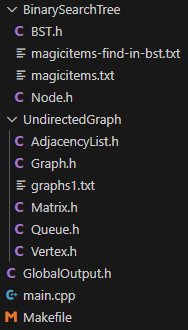
\includegraphics[width=0.25\textwidth]{./imgs/ProgramDirectories.PNG}}
    \caption{Program Directories}
    \label{fig:figure1.3}
\end{figure}

\section{Undirected Graph}
\setcounter{figure}{0} % Reset figure counter

\subsection{File Parser and Keywords}
\noindent
The first implementations I will explain for this program is the undirected graph implementations. For this section, I created three implementations of the undirected graph, which are as a matrix, as an adjacency list, and as linked objects. These three implementation types will be explained later in this section. 

\vspace{1em}

\noindent
What made this section of the assignment difficult was the parser I had to create in order to read in the graph file. The graphs1.txt file had all the vertices and edges I had to create. With each graph in the file, I needed to make a version for the matrix, a version for the adjacency list, and a version for the linked objects. In order to create these versions, I had to have my program read each line and figure out what to do. Below in Figure 2.1 is an example snippet of the graph file, showing only one graph being created with all of its vertices and edges.

\begin{figure}[H]
  \centering
  \lstinputlisting[firstline=1, firstnumber=1, lastline=20]{UndirectedGraph/graphs1.txt} 
  \caption{Section of Graph Creation File (graphs1.txt)}
  \label{fig:figure2.1}
\end{figure}

\noindent
I had to read this file and understand all the keywords that were being used in order to create a parser and do tokenization based on each line in the file. Below is how I created a parser for the graph file, as well as calling the appropriate functions to create the undirected graphs, matrices, and more.

\begin{figure}[H]
  \centering
  \lstinputlisting[firstline=27, firstnumber=27, lastline=28]{main.cpp} 
  \label{fig:figure2.2-part1}
\end{figure}

\begin{figure}[H]
  \centering
  \lstinputlisting[firstline=34, firstnumber=34, lastline=38]{main.cpp} 
  \label{fig:figure2.2-part2}
\end{figure}

\begin{figure}[H]
  \centering
  \lstinputlisting[firstline=49, firstnumber=49, lastline=87]{main.cpp} 
  \label{fig:figure2.2-part3}
\end{figure}

\begin{figure}[H]
  \centering
  \lstinputlisting[firstline=88, firstnumber=88, lastline=123]{main.cpp} 
  \caption{File Parsing for Undirected Graph (main.cpp)}
  \label{fig:figure2.2-part4}
\end{figure}

\noindent
The file reading variable I created in order to make the parser work is the "file" variable, declared on Line 28, which stores the input file (in this case, it is graphs1.txt by Lines 50-55, but this file variable is also used by the Binary Search Tree code, which will be explained later). Other variables I used were:

\begin{itemize}
    \item (Line 35) The myGraph variable, which is a pointer to an instance of the Graph class, which will be explained in depth in a future section. This variable stores the Graph being worked on currently.
    \vspace{1em}
    \item (Line 36) The myMatrix variable, which is a pointer to an instance of the Matrix class, which will be explained in depth in a future section. This variable stores the Matrix being worked on currently.
    \item (Line 37) The check variable, which is a boolean that stores whether or not information about a Graph needs to be printed. It's almost always true, except for the first instance of a new graph being created.
    \item (Line 38) The curGraphNum variable, which is an integer that stores the current graph number to make the display look better when the information needs to be printed.
    \item (Line 60) The currentWord variable, which initially takes the first word of each line (labeled as command) as the code runs through each line of the file (Loop at Line 58). Throughout the parser, it will go to the next word on that same line, and then to the next and next if it needs to to gather more information.
    \item (Line 61) The word variable, which is a string that takes the value of the currentWord variable and uses it throughout the if statements in the parser.
    \item (Line 61) The nextWord variable, which takes the word after the "word" variable in the file on that same line (which will be given by the currentWord, kind of confusing to explain but it works, so trust me)
    \item (Line 61) The vertexID variable, which is a string that deal with the vertices when adding a Vertex to the Graph. This will be explained more in depth later in this section.
    \item (Line 61-62) The vertex1 and vertex2 strings, and the vertex1Index and vertex2Index integers, which all deal with the vertices when adding an Edge. These will be explained more in depth soon.
\end{itemize}

\noindent
To create a parser, I needed to find out the possible options for each command. The two words that the commands can start with are "new" or "add", and I would have to ignore anything else. When iterating through each line of the file (Line 58), I would iterate again over each word on each line (Line 65). 

\begin{itemize}
    \item If the current word was "--", that means that it is a comment, so this line would be skipped and go straight to the next line (Lines 68-71).
    \item If the current word was "new", that means that a new Graph and a new Matrix would need be created (the adjacency list is not yet created, as it is created all the way at the end after the Graph and Matrix are finished being altered and added to). The printInformation function will run (explained in the next section), the check boolean gets set to true, and a new Graph and Matrix are created and stored in the variables myGraph and myMatrix respectively (Lines 73-87).
    \item If the current word was "add", that means either a vertex or edge needs to be added (Line 89). The program will then check the next word in the file to find out what to add to the Graph (Line 92).
    \begin{itemize}
        \item If the next word after "add" is "vertex", that means a vertex needs to be added. For this specific file, the format for adding a vertex is "add vertex $n$", where $n$ is the vertex ID of the Vertex being added. The program gets that vertex ID, and adds a vertex to the Graph class. It also will increment the size of the Matrix by one and pass that vertex ID to the Matrix class, since a new Vertex got added. Again, for clarity, these classes will be explained in depth in future sections (Lines 93-98).
        \item If the next word after "add" is "edge" (Line 100), that means an edge needs to be added. For this specific file, the format for adding a vertex is "add edge $n_1$ - $n_2$", where $n_1$ is the first vertex ID and $n_2$ is the second vertex ID. In the program, $n_1$ is represented by the string vertex1 (Line 103), and $n_2$ is represented by the string vertex2 (Line 104), making sure to skip over the "-" before getting the second vertex ID. An edge needs to be added between these two vertices, so the program calls a function to get the indices of these vertices in the Graph class (Lines 107-108), WHICH WILL BE EXPLAINED SOON I PROMISE. and it will call another Graph class function to add an edge between these two indices (Line 111). It will then also set the Matrix value to 1 at these same indices for the Matrix class (Line 114). 
    \end{itemize}
\end{itemize}

\noindent
This input file will then be closed to make sure no memory leaks will occur regarding the file (Line 120). After this, the printInformation function is called one last time to print the final graph on Line 123. 

\vspace{0.5em}
\noindent
Because the program assumes all vertices will be added before any edges would be added, as shown in the graphs1.txt file, incrementing the size of the Matrix won't interfere with setting the Matrix values. It also wouldn't interfere with adding edges for the Graph class.

\vspace{0.5em}
\noindent
The parser took the majority of my time to create because it was a lot of work to learn how the istringstream data type worked for the currentWord variable. The istringstream data type allows for reading from a string as if it were a stream. In my case, I used it to break down a string into tokens for separating each word on each line in the file.

\subsection{PrintInformation Output Function}
\noindent
The print information output function is a function that appears in the main file that will print the Matrix table, the Adjacency List, and the depth-first and breadth-first traversals of the linked objects. This is also the function that will unload the objects in memory since they will be replaced by a new Graph/Matrix or no new Graph is created so it is used to free memory. 

\vspace{1em}
\noindent
Below is the implementation of the printInformation function.

\begin{figure}[H]
  \centering
  \lstinputlisting[firstline=15, firstnumber=15, lastline=16]{main.cpp} 
  \label{fig:figure2.3-part1}
\end{figure}

\vspace{-2em}

\begin{figure}[H]
  \centering
  \lstinputlisting[firstline=186, firstnumber=186, lastline=221]{main.cpp} 
  \caption{printInformation function (main.cpp)}
  \label{fig:figure2.3-part2}
\end{figure}

\noindent
The first printInformation "call" actually isn't a call at all, but it is a prototype. Since the function takes place after the code of the main() function, there needs to be a prototype function that makes the program know that the printInformation function will be coming (Line 16).

\vspace{1em}

\noindent
The printInformation function takes in four parameters.
\begin{itemize}
    \item The needToPrint parameter is the check variable, which checks whether or not the results need to be printed.
    \item The graphNum parameter is the curGraphNum variable, which keeps track of which graph the program is currently on. The "\&" indicates that any updates to the graphNum variable will also update the curGraphNum because it is being passed by reference instead of passed by value. The graph number will always start at 1 (no such thing as Graph \#0, sorry!) 
    \item The matrix and graph parameters and myMatrix and myGraph respectively, which are pointers that hold all the information about the current Graph and Matrix.
\end{itemize}

\noindent
The function first checks if it needs to print anything (Line 188). This would only fail if the function is called and no graph has been created yet. If it's true, however, the current graph number would be incremented (Line 190) and since the parameter was passed by reference, the curGraphNum variable would also update. 

\vspace{1em}
\noindent
The Matrix is then printed using a Matrix function called printMatrix (Lines 193-195). 

\vspace{1em}
\noindent
After this, the Adjacency List is printed using a global function called printAdjacencyList, located in the header file AdjacencyList.h, which takes the graph as a parameter (Lines 198-200). Like mentioned briefly earlier, the adjacency list is only created after the Graph and Matrix are finished being built. This is because the adjacency list uses the actual Graph to determine what values to print. 

\vspace{1em}
\noindent
After these implementations are printed to the outFile, the depth-first traversal and the breadth-first traversal are printed for the linked objects Graph implementation (Lines 203-206, 212-215). The checkDFT function on Line 206 and checkBFT function on Line 215 are for those vertices that aren't connected to the first vertex, since the traversals start at the first Vertex of the Graph. It is also important to note the Graph function labeled resetProcessed, which resets all the processed values of each Vertex so another traversal can be done on the same Graph (Line 209).

\vspace{1em}
\noindent
The Graph and Matrix then need to be unloaded to avoid any memory leaks or errors, so they are unloaded at the end of this function (Lines 219-221).

\subsection{Implementing Graph as Matrix}
\noindent
My implementation of the Matrix class is found in the Matrix.h file in the UndirectedGraph directory. Figure 2.4 below shows the members of the Matrix class.

\begin{figure}[H]
  \centering
  \lstinputlisting[lastline=14]{UndirectedGraph/Matrix.h} 
  \caption{printInformation function (Matrix.h)}
  \label{fig:figure2.4}
\end{figure}

\noindent
The two members of the Matrix class are the two-dimensional vector of the actual matrix and the vertexIDs vector. Instead of making the matrix a 2D array, I made it a 2D vector since the size of the vector will change a lot throughout the program. I am dynamically allocating more memory for the matrix. The vertexIDs vector will store all of the IDs of the vertices in the Graph, which is very similar to the vertices member of the Graph class that will be explained later. The reason why I made these separate variables, even though they contain exactly the same information, is because I wanted to separate the Matrix and Graph classes and I didn't want them to rely on each other's members.

\vspace{1em}
\noindent
Below is the implementation of the incrementSize function, which increments the size of the matrix every time a new Vertex is added.

\begin{figure}[H]
  \centering
  \lstinputlisting[firstline=16, firstnumber=16, lastline=27]{UndirectedGraph/Matrix.h} 
  \caption{incrementSize function (Matrix.h)}
  \label{fig:figure2.5}
\end{figure}

\noindent
The function begins by adding the new vertex ID to the end of the vertexID vector (Line 19). It then resizes the matrix to be the size of the vertexID vector (Line 20-22). Each row of the matrix is then resized to ensure that the 2D vector is square, with the new entries being initialized to 0 to prevent garbage values in the matrix (Lines 23-26). This was an issue I had for a long time until I realized I'm resizing the array without giving the new indices any proper value. 

\vspace{1em}
\noindent
Below is the implementation of the addValue function, which sets the value to 1 at a specified element.

\begin{figure}[H]
  \centering
  \lstinputlisting[firstline=29, firstnumber=29, lastline=34]{UndirectedGraph/Matrix.h} 
  \caption{addValue function (Matrix.h)}
  \label{fig:figure2.6}
\end{figure}

\noindent
The parameters indicate which element to change in the matrix 2D vector. The value of the i-th row and j-th column, and also the value of the j-th row and i-th column, are changed. The reason why they are both changed is because this graph is an undirected graph, meaning any edge connecting two vertices has that edge connecting from vertex1 to vertex2, and also vertex2 to vertex1. There is no arrowhead on the edge when it comes to undirected graphs. This also means the result of the matrix table will be symmetrical across the diagonal line from matrix[First Vertex][First Vertex] to matrix[Last Vertex][Last Vertex] in the matrix table output.

\vspace{1em}

\noindent
The final function of the Matrix class is the printMatrix function, which prints the Matrix to the outFile.

\begin{figure}[H]
  \centering
  \lstinputlisting[firstline=36, firstnumber=36, lastline=55]{UndirectedGraph/Matrix.h} 
  \label{fig:figure2.7-part1}
\end{figure}

\begin{figure}[H]
  \centering
  \lstinputlisting[firstline=56, firstnumber=56]{UndirectedGraph/Matrix.h} 
  \caption{printMatrix function (Matrix.h)}
  \label{fig:figure2.7-part2}
\end{figure}

\noindent
This function has an interesting feature where the vertexIDs for the matrix can either be displayed or not displayed depending on if the boolean "displayIDs" is set to true or false. This option will be explained later, but if it is on, the vertexIDs will be displayed as the first row and first column, but if it is off, they won't be displayed, and only the matrix elements will be displayed. The function really begins by getting the size of the rows and columns of the matrix in order to know how many times to do the iterations when printing the matrix table (Line 40). The function then prints the first row of the matrix table, which are all of the IDs listed in the vertexIDs vector if the displayIDs boolean is set to true (Lines 43-51). Then, it will print out all of the elements from the matrix, including the vertexIDs as the first element in each row if that boolean is set to true.  

\vspace{1em}

\noindent
For this specific matrix implementation, I added a snippet of code from Lines 62-65 where if the vertex ID of that column is larger than just one letter or number, it would add an extra space so the column can align with the correct row it is supposed to be paired to. This would only work in the case of if the vertex ID of the column being 2 letters or numbers long, as is the case in graphs1.txt. There is no vertex ID in that text file that is over 2 characters long. This is obviously something that shouldn't be assumed since any file with the correct command format can be used, but there wouldn't be any easily accessible and feasible way to nicely format and display the matrix table if the IDs are all different lengths. Of course there are ways, but that takes away from the focus of this program. This is why I added the "displayIDs" boolean. If the output of the matrix looks ugly if running it with another file, then set the boolean to false to remove the vertexID row and column.  

\vspace{2em}

\noindent
Below are example images that display the Matrix output of the first Graph and the fifth Graph in graphs1.txt:

\begin{figure}[H] 
    \centering 
    \fbox{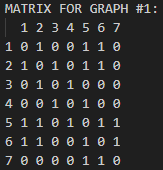
\includegraphics[width=0.4\textwidth]{./imgs/MatrixGraph1.PNG}}
    \caption{Graph \#1 Matrix}
    \label{fig:figure2.8}
\end{figure}

\begin{figure}[H] 
    \centering 
    \fbox{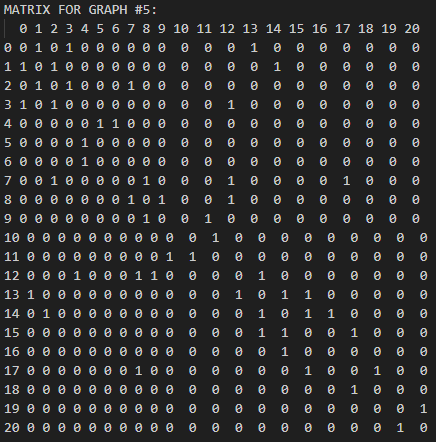
\includegraphics[width=0.6\textwidth]{./imgs/MatrixGraph5.PNG}}
    \caption{Graph \#5 Matrix}
    \label{fig:figure2.9}
\end{figure}

\noindent
As is shown in the images above, the matrix is a binary matrix, so the result will be either 0 or 1. Apologies for the spacing issue at the row with the vertex of ID 10 in Graph \#5. However, it is still very easy to read to what column the element corresponds to, even with that spacing shift. Because this issue could be worse with longer vertex IDs, it is recommended to set the "displayIDs" boolean to false if dealing with a graph file that has longer vertex IDs.

\subsection{Vertex Class}
\noindent
In order to explain the implementation of an undirected graph as linked objects, I need to explain the Vertex class. A Vertex is the actual "Node" that is in the undirected graph. These nodes are connected to each other by edges. Below is how I implemented this class

\begin{figure}[H]
  \centering
  \lstinputlisting[]{UndirectedGraph/Vertex.h} 
  \caption{Vertex Class (Vertex.h)}
  \label{fig:figure2.10}
\end{figure}

\noindent
The members of the Vertex class are:
\begin{itemize}
    \item id, which is a string that stores the ID of the Vertex (Line 11). This is the same concept of the IDs of the vertices in the Matrix discussed in the previous section.
    \item processed, which is a boolean that says whether or not it has been processed by either the depth-first or breadth-first traversal (Line 12). This is to make sure this Vertex isn't printed multiple times in the output of the same traversal. This processed value is reset between every traversal function call.
    \item neighbors, which is a vector of Vertices that stores the one-hop neighbors of this Vertex (Line 13). If there is an edge connecting this Vertex to another, that Vertex will be in the neighbors vector.
    \item next, which points to another Vertex (Line 16). It is only used for the breadth-first traversal Queue, which will be explained later.
\end{itemize}

\noindent
This class has a parameterized constructor, used when each Vertex is created in the Graph class. It sets the ID of the vector to the parameter that was passed into by the function (Lines 19-22).

\vspace{1em}

\noindent
This is also one function tied to this class, which is the addNeighbor function. This function adds a neighbor to this vertex by appending the one-hop neighboring Vertex (the parameter passed in to the function by reference) to the neighbors vector for the current Vertex (Lines 25-28).

\subsection{Queue Class}
\noindent
The single purpose of the Queue class for this assignment is to aid in the breadth first traversal for the linked objects implementation of the Graph. This class is exactly the same as it was in Assignment 1, except now, instead of using the Node class, I am using the Vertex class. Below is my implementation of the Queue class:

\begin{figure}[H]
  \centering
  \lstinputlisting[lastline=26]{UndirectedGraph/Queue.h} 
  \label{fig:figure2.11-part1}
\end{figure}

\begin{figure}[H]
  \centering
  \lstinputlisting[firstline=27, firstnumber=27]{UndirectedGraph/Queue.h} 
  \caption{Queue Class (Queue.h)}
  \label{fig:figure2.11-part2}
\end{figure}

\noindent
The two members for the Queue class are the head and tail, which are of the Vertex class. The head points to the first Vertex in the linked list, while the tail points to the last Vertex in the linked list (Lines 13-14). The "next" member of the Vertex class is used for this Queue. The three functions for this class are:
\begin{itemize}
    \item enqueue, which adds a new Vertex to the back of the linked list (Lines 17-30)
    \item dequeue, which removes the head of the linked list and is returned (Lines 33-44)
    \item isEmpty, which checks if the queue is empty or not (Lines 47-50) 
\end{itemize}

\subsection{Implementing Graph as Linked Objects}
\noindent
The Vertex and Queue classes are the fundamentals of the Graph class (especially the Vertex class, since the Queue class is only used for one function). Below is how I implemented the vertices member for the Graph class:

\begin{figure}[H]
  \centering
  \lstinputlisting[lastline=17]{UndirectedGraph/Graph.h} 
  \caption{Graph Class Member (Graph.h)}
  \label{fig:figure2.12}
\end{figure}

\noindent
The vertices member is a vector of all Vertices in the entire graph (Line 17). This vector will be used a lot in the upcoming functions regarding the Graph and its traversals.

\vspace{1em}

\noindent
The first function of the Graph class is the addVertex function, as shown below.

\begin{figure}[H]
  \centering
  \lstinputlisting[firstline=19, firstnumber=19, lastline=24]{UndirectedGraph/Graph.h} 
  \caption{addVertex (Graph.h)}
  \label{fig:figure2.13}
\end{figure}

\noindent
This function will add a Vertex to the Graph. It does this by creating a new Vertex from the Vertex class with the ID that was passed into the function (Line 22), and then it adds that Vertex to the vertices list for the Graph (Line 23).

\vspace{1em}
\noindent
The next function of the Graph class is the findVertexIndex function, as shown below.

\begin{figure}[H]
  \centering
  \lstinputlisting[firstline=26, firstnumber=26, lastline=29]{UndirectedGraph/Graph.h} 
  \label{fig:figure2.14-part1}
\end{figure}

\begin{figure}[H]
  \centering
  \lstinputlisting[firstline=30, firstnumber=30, lastline=38]{UndirectedGraph/Graph.h} 
  \caption{findVertexIndex (Graph.h)}
  \label{fig:figure2.14-part2}
\end{figure}

\noindent
The findVertexIndex function returns an index that matches a Vertex with a specific ID in the vertices array. This function is used to get the index for adding edges in the main parser. The function does a linear search through the vertices array to find the correct Vertex to return. It does this by iterating through the vertices array (Line 29) and it checks if the ID of the current iterated Vertex is equal to the specific ID from the parameter (Line 31). If it is equal, the function returns that index for the parser to use (Line 33). If no vertex ID is found in the vertices array, a runtime error will occur because the function assumes that the a correct Vertex ID will be found (Line 37). The only way to get out of the function without any errors is if a some Vertex is found.

\vspace{1em}
\noindent
The next function of the Graph class is the addEdge function, as shown below.
\begin{figure}[H]
  \centering
  \lstinputlisting[firstline=40, firstnumber=40, lastline=45]{UndirectedGraph/Graph.h} 
  \caption{addEdge (Graph.h)}
  \label{fig:figure2.15}
\end{figure}

\noindent
The purpose of the addEdge function is to add an edge between two Vertices. The two parameters for this function are two indices that are returned from the findVertexIndex function. This means that vertices[vertex1] and vertices[vertex2] are the Vertices with the IDs specified from the parser. The function will add vertex2 as a neighbor to vertex1 (Line 43) and will add vertex1 as a neighbor to vertex2 (Line 44). They are both neighbors of each other because it is an undirected graph. If the graph was directed, the order between the two parameters would matter, kind of like adding a value for the Matrix.

\vspace{1em}
\noindent
Before explaining the traversals, I want to explain the function resetProcessed for the Graph class, as shown below.
\begin{figure}[H]
  \centering
  \lstinputlisting[firstline=83, firstnumber=83, lastline=89]{UndirectedGraph/Graph.h} 
  \caption{resetProcessed (Graph.h)}
  \label{fig:figure2.16}
\end{figure}

\noindent
This function sets the processed value for all vertices to false. The traversal functions change the processed values to true for the vertices, so resetting it allow for other traversal to be ran. This function is called between the depth-first traversal and the breadth-first traversal. This function does this by iterating through the vertices array and setting the processed member of each Vertex to false (Lines 85-88).

\vspace{1em}
\noindent
The last function I want to explain before explaining the traversals is the unloadGraph function, which is called after all information is printed. This function is shown below.

\begin{figure}[H]
  \centering
  \lstinputlisting[firstline=91, firstnumber=91, lastline=102]{UndirectedGraph/Graph.h} 
  \caption{unloadGraph (Graph.h)}
  \label{fig:figure2.17}
\end{figure}

\noindent
The function iterates through each Vertex in the vertices vector and deletes it (Lines 95-98). It then clears the vertices vector to make sure no extra memory leaks, just in case (Line 101).

\vspace{1em}
\noindent
The final functions for this class are for depth-first traversal and breadth-first traversal. However, there are two separate functions for each. The public functions the parser call are named depthFirstTrav and breadthFirstTrav, which then call the private functions DFT and BFT respectively, as shown below.

\begin{figure}[H]
  \centering
  \lstinputlisting[firstline=47, firstnumber=47, lastline=51]{UndirectedGraph/Graph.h} 
  \label{fig:figure2.18-part1}
\end{figure}

\vspace{-3em}

\begin{figure}[H]
  \centering
  \lstinputlisting[firstline=65, firstnumber=65, lastline=69]{UndirectedGraph/Graph.h} 
  \caption{Public functions depthFirstTrav and breadthFirstTrav (Graph.h)}
  \label{fig:figure2.18-part2}
\end{figure}

\noindent
The DFT and BFT function calls in each of these public functions have parameters, which signify that the traversals will start from the root node. The main reason why I made these two separate functions are for readability. I didn't want to have the code line like "graph-$>$DFT(graph-$>$vertices[0])" in my printInformation function in main because it looks very clunky. Instead, the line of code is just "graph->depthFirstTrav();", which looks a lot cleaner than the other line (shown on Line 205 of Figure 2.3). I perform a similar action when doing traversals for the BST as well.

\vspace{1em}

\noindent
Below is my implementation of the Depth-First Traversal private function for the linked objects.
\begin{figure}[H]
  \centering
  \lstinputlisting[firstline=105, firstnumber=105, lastline=121]{UndirectedGraph/Graph.h} 
  \caption{DFT (Graph.h)}
  \label{fig:figure2.19}
\end{figure}

\noindent
Depth-first traversal prioritizes going deep before going wide. This ideology can be achieved by using recursion. The implicit runtime stack of the return addresses can be the data structure that helps with this. This function begins by checking if the current Vertex is processed. If it is not processed, the Vertex ID will be printed and that specific Vertex will be processed (Line 108-112). It will then iterate through each neighbor of the current Vertex, and if the current neighbor isn't processed, it will make a recursive call for DFT (Lines 114-120). The function explores each Vertex by going as deeply as possible into its neighbors before backtracking, rather than visiting all neighbors at the same level first.

\vspace{1em}
\noindent
Below is my implementation of the Breadth-First Traversal private function for the linked objects.
\begin{figure}[H]
  \centering
  \lstinputlisting[firstline=123, firstnumber=123]{UndirectedGraph/Graph.h} 
  \caption{BFT (Graph.h)}
  \label{fig:figure2.20}
\end{figure}

\noindent
Breadth-first traversal prioritizes going wide before going deep. This ideology can be achieved by using the Queue class. This function begins by creating a new Queue, enqueuing the current Vertex to the queue, and processing it (Lines 129-131). The function then will loop until the Queue becomes empty, and in the loop the first Vertex in the Queue will be dequeued and printed to the output (Lines 133-136). It will then iterate through the neighbors of that dequeued Vertex and add each neighbor to the Queue if it hasn't been processed, also setting the neighbor's processed value to true (Lines 137-146). Once all non-processed neighbors are added to the queue, the function will then go to the beginning of the loop, dequeue the first one, print it, and then iterate through its neighbors. Once all values have been processed and the Queue is empty, the Queue is deleted from memory and the function ends (Line 148). Basically, the function visits all neighbors at the same level first, rather than exploring each Vertex by going as deeply as possible into its neighbors.

\vspace{1em}
\noindent
The last two functions to explain are the checkDFT and checkBFT functions, which are used in order to see if there were any unconnected Vertices to the root Vertex. If there were, it wouldn't have been printed when doing the original DFT/BFT, so a function would have to help with this, functions which are shown below.

\begin{figure}[H]
  \centering
  \lstinputlisting[firstline=53, firstnumber=53, lastline=63]{UndirectedGraph/Graph.h} 
  \label{fig:figure2.21-part1}
\end{figure}

\vspace{-3em}

\begin{figure}[H]
  \centering
  \lstinputlisting[firstline=71, firstnumber=71, lastline=81]{UndirectedGraph/Graph.h} 
  \caption{Traversal Check Functions (Graph.h)}
  \label{fig:figure2.21-part2}
\end{figure}

\noindent
These functions are the exact same thing, except for the function call in the loop. The functions work by iterating through the vertices vector, and if the current vector has not been processed, start either a DFT or BFT with that vector as the root (Lines 56-62, 74-80). 

\vspace{2em}
\subsection{Asymptotic Running Time of Graph Traversals}

\noindent
It is important to note the time complexity of the Depth-First Traversal and Breadth-First Traversal when working with the implementation with linked objects. The time complexity of both DFT and BFT is $O(|V| + |E|)$, where $V$ represents the set of Vertices in the graph, and $E$ represents the set of Edges in the graph. The $||$ represent the cardinality of the sets, so the time complexity of these traversals is the number of vertices + number of edges. This is because in the worst case, for both traversals, each vertex and each edge are visited once. It is hard to prove through output that this is accurate since no comparison number is being counted, unlike last assignment. However, here is the output for the traversals for Graph \#1 and Graph \#5.

\begin{figure}[H] 
    \centering 
    \fbox{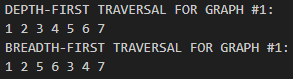
\includegraphics[width=0.6\textwidth]{./imgs/TraversalsGraph1.PNG}}
    \caption{Graph \#1 Traversals}
    \label{fig:figure2.22}
\end{figure}

\begin{figure}[H] 
    \centering 
    \fbox{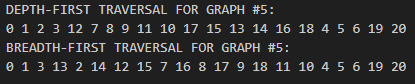
\includegraphics[width=0.6\textwidth]{./imgs/TraversalsGraph5.PNG}}
    \caption{Graph \#5 Traversals}
    \label{fig:figure2.23}
\end{figure}

\noindent
There is no specific reason why I keep using the Graph 1 and Graph 5, other than that the outputs are concise and get to the point. All vertices are visited for each traversal, including those that may not be connected to any other Vertex. Each vertex and edge may be visited once, so that's why the time complexity of these traversals is $O(|V| + |E|)$.

\subsection{Implementing Graph as Adjacency List}
\noindent
The final implementation of the undirected graph is the adjacency list, which is probably the easiest implementation of them all because it borrows aspects from the linked objects implementation by using the Graph class. There is only one function that deals with the adjacency list, called printAdjacencyList (located in AdjacencyList.h), which takes the current Graph as a parameter. This function is called in the printInformation main function, and is shown below.

\begin{figure}[H]
  \centering
  \lstinputlisting[]{UndirectedGraph/AdjacencyList.h} 
  \caption{printAdajcencyList function (AdjacencyList.h)}
  \label{fig:figure2.24}
\end{figure}

\vspace{-1em}
\noindent
The function begins by declaring some variables.
\begin{itemize}
    \item The graphVertices vector, which points to the vertices from the Graph class (Line 14)
    \item The size integer, which gets the size of the vertices vector (Line 15)
    \item The neighborSize variable is declared, which eventually will get the size of the current Vertex neighbors member, which facilitates the process of looping through the neighbors of the current Vertex(Line 16)
    \item The Vertex named currentVertex and the currentNeighborID string are declared, which will be used in the loops coming soon (Lines 18-19)  
\end{itemize}

\noindent
The function iterates through each Vertex in the Graph, as the adjacency list needs to print out the neighbors for each Vertex (Line 22). The ID of that Vertex is printed (Line 28) and then an inner loop iterates through the neighbors of that Vertex, printing them each one by one (Lines 31-35).

\vspace{1em}
\noindent
Below are the adjacency lists of Graph \#1 and Graph \#5, showing the proper format of a list.

\begin{figure}[H] 
    \centering 
    \fbox{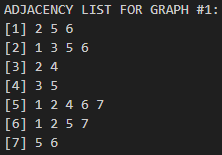
\includegraphics[width=0.4\textwidth]{./imgs/ListGraph1.PNG}}
    \caption{Graph \#1 Adjacency List}
    \label{fig:figure2.25}
\end{figure}

\begin{figure}[H] 
    \centering 
    \fbox{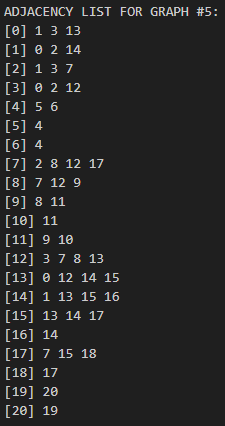
\includegraphics[width=0.3\textwidth]{./imgs/ListGraph5.PNG}}
    \caption{Graph \#5 Adjacency List}
    \label{fig:figure2.26}
\end{figure}

\noindent
As shown in the images above, the vertex IDs are printed within the brackets, and each neighbor of that Vertex is printed in its row.

\section{Binary Search Tree}
\setcounter{figure}{0} % Reset figure counter

\subsection{BST Main Function Calls}
\noindent
A Binary Search Tree, or BST, is a type of binary tree. Each node on the tree must have 0, 1, or 2 child nodes. The child nodes are called "left" and "right" nodes. The left child contains values less than the parent node and the right child contains values greater than (or equal to) the parent node. In this case, since I will be using the magic items, the data is a string, so they will be in ASCII order. Below shows opening the magicitems.txt file and inserting each item from the file into the BST. 

\begin{figure}[H]
  \centering
  \lstinputlisting[firstline=27, firstnumber=27, lastline=32]{main.cpp} 
  \label{fig:figure3.1-part1}
\end{figure}

\vspace{-3em}

\begin{figure}[H]
  \centering
  \lstinputlisting[firstline=130, firstnumber=130, lastline=146]{main.cpp} 
  \caption{Call to Insert Items into BST (main.cpp)}
  \label{fig:figure3.1-part2}
\end{figure}

\vspace{-1em}
\noindent
The section of code starts off by reading the magicItems.txt file successfully (Line 131-136). Then, each magic item in the file is read and then inserted into the BST (Line 140-143). The path each item took for the insertions are printed out using this function. The BST is declared at the beginning of the program (Line 32) using the BST class object, which will be explained later. The magicitems file is then closed since another file will need to be read eventually (Line 146). Below shows the next step for the BST, which would be calling the function to print out an in-order traversal.

\begin{figure}[H]
  \centering
  \lstinputlisting[firstline=148, firstnumber=148, lastline=150]{main.cpp} 
  \caption{Call to Print BST In-Order Traversal (main.cpp)}
  \label{fig:figure3.2}
\end{figure}

\noindent
The function above does all the work for the in-order traversal, as will be explained soon (Line 150).

\vspace{1em}
\noindent
After the in-order traversal is printed to the output file, it is time for the BST lookups. The file "magicitems-find-in-bst.txt" holds 42 different items that are found in the magic items file, meaning those values will be in the BST. Below is the implementation of the BST function calls from main for this step.

\begin{figure}[H]
  \centering
  \lstinputlisting[firstline=152, firstnumber=152, lastline=172]{main.cpp} 
  \caption{Function calls for BST lookups (main.cpp)}
  \label{fig:figure3.3}
\end{figure}

\noindent
First, the magicitems-find-in-bst file gets opened up successfully (Lines 153-158). Then, each item of that file is read and searched for in the BST (Lines 163-170). The number of comparisons it took for each lookup is printed alongside the path it took to find that item. The comparison count will be tallied up using the "avg" variable (Line 168), like how the binary search comparison counts were tallied up in the previous assignment. The average comparison count for all BST lookups will be explained in a future section. 

\subsection{Node Class}
\noindent
For items to be inserted into the BST, they need to be created as Nodes first. Nodes are the objects that are connected to each other in the tree. Below is my implementation of the Node class used for the BST.

\begin{figure}[H]
  \centering
  \lstinputlisting[]{BinarySearchTree/Node.h} 
  \caption{Node Class (Node.h)}
  \label{fig:figure3.4}
\end{figure}

\noindent
The Node is very similar to the Nodes used for the linked list implementations for the Stack and Queue back in Assignment 1, and even some members of the Vector class can relate to this. It has a string member, which would be the name of the magic item (Line 13). Unlike the previous Nodes, instead of a next pointer, which would point to another Node, there are two pointers that point to child Nodes, labeled left and right (Lines 16-17). There is also a Node constructor, which is called when a new Node is created when inserting a Node into the BST (Lines 20-25). This sets the data of the Node to be the name of the magic item. The left and right pointers will be manipulated in the process of insertion.   

\subsection{Inserting into BST}
\noindent
After explaining the Node class, it is almost time to explain the functions of the BST class. However, first, I want to explain the one member of this class, which is the root shown below.

\begin{figure}[H]
  \centering
  \lstinputlisting[lastline=13]{BinarySearchTree/BST.h} 
  \caption{Root Member of BST (BST.h)}
  \label{fig:figure3.5}
\end{figure}

\vspace{-0.5em}
\noindent
The root member is a pointer that points to the Node that is the root of the tree. This root is used for all of the functions in the class since it is the Node that is the starting place for operations like insertion and searching, as will be shown.

\vspace{0.5em}
\noindent
It is now time to talk about the first function of the BST class, which is insertion.

\vspace{-1em}
\begin{figure}[H]
  \centering
  \lstinputlisting[firstline=15, firstnumber=15, lastline=33]{BinarySearchTree/BST.h} 
  \label{fig:figure3.6-part1}
\end{figure}

\begin{figure}[H]
  \centering
  \lstinputlisting[firstline=34, firstnumber=34, lastline=73]{BinarySearchTree/BST.h} 
  \caption{Insert a Node into BST (BST.h)}
  \label{fig:figure3.6-part2}
\end{figure}

\noindent
The function begins by initializing some variables, which are:
\begin{itemize}
    \item newNode, which is the Node that will be inserted into the BST (Line 20)
    \item prev, which is the Node that will be the "parent" of the new Node (Line 21)
    \item curNode, which is the Node that finds the correct path to insert the new Node (Line 22)
    \item lessThan, which is a boolean that keeps track if the new Node should be a left child or the right child of the "prev" Node (Line 23)
\end{itemize}

\noindent
The function will then try to find the correct spot to insert the new Node. The curNode, which starts at the root of the tree, will be changed each iteration of the while loop. The loop will continue until it has found a leaf node of the tree, meaning there is no more tree to traverse (Line 29). In the loop, the prev Node will be set (Line 33). Again, this will be the parent of the inserted Node. When doing insertions, this function will print the path it took to get to wherever the Node needed to be inserted (Ex: L, R, L, L, etc). Lines 35-38 are just for readability of the output, making sure it doesn't print a comma before any letter is printed. The last part of this loop checks which way to go down the tree. If the Node belongs in the left sub-tree, meaning its ASCII value is smaller than the current Node's item, it will print an L, set the boolean to say it is smaller than current Node (will be used later), and the loop will continue with the current Node being the left child of the previous current Node (Lines 41-46). However, if this is not the case, that means that the Node belongs in the right sub-tree, meaning its ASCII value is greater than or equal to the current Node's item. It will print an R, set the boolean to say it is larger than the current Node, and the loop will continue with the current Node being the right child of the previous current Node (Lines 48-53). 

\vspace{1em}
\noindent
The loop is exited once the current Node is NULL, meaning it has made it the leaf Nodes of the tree. Once this happens, that means that the "prev" Node has been set to the leaf Node which will now be the parent of the new Node. If the loop was never iterated through, meaning the root Node was NULL, the new Node will be the root of the tree (Lines 57-60). This only happens during the first insertion of a brand new tree. However, if it's not the root of the tree, and the loop was iterated through, that means that the program needs to determine whether it should be the left child or right child of the "prev" Node. This is where the "lessThan" boolean comes into place. If the new Node's item is smaller than the prev Node's item, the new Node will be the left child of its parent (Lines 62-65). If it is not, then the new Node will be the right child of its parent (Lines 67-70).

\vspace{1em}
\noindent
The time complexity of inserting a new Node into the BST is actually very similar to the time complexity of looking up a Node in the BST. As it will be shown, the overall ideas between the two functions are actually very similar. In that case, I will be showing its time complexity when explaining the search function for the BST.

\vspace{5em}
\noindent
Below is an image that displays the beginning of the BST insertion output.

\begin{figure}[H] 
    \centering 
    \fbox{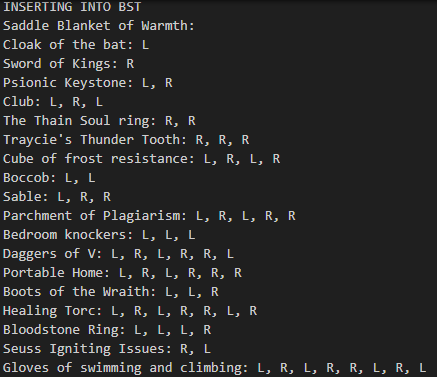
\includegraphics[width=0.6\textwidth]{./imgs/InsertionBST.PNG}}
    \caption{Snippet of BST Insertion Output}
    \label{fig:figure3.7}
\end{figure}

\noindent
As it is evident, the first item inserted into the BST has no path. This is because it is the root. The rest of the insertions have paths from the root Node. For example, since 'Cloak of the bat' is smaller than 'Saddle Blanket of Warmth', it belongs in its left subtree, which is shown by the its output being an 'L'. When the tree gets larger there is a lot more output for its paths. It is also important to note that there is no code to make the tree balanced. There is no AVL balancing being practiced, so there is a chance that this tree can be unbalanced, which could be horrific for its time complexity, but this will all be explained when testing the running time for the traversals and BST lookups. 

\subsection{In-order Traversal of BST}
\noindent
Like with the undirected graph traversal functions, there are two separate functions for the in-order traversal, one is public while the other is private. The public function, named inorderTrav, is called by main (as shown on Line 150 of Figure 3.2). This public function then calls the private function named inorderBST, as shown below. 

\begin{figure}[H]
  \centering
  \lstinputlisting[firstline=75, firstnumber=75, lastline=79]{BinarySearchTree/BST.h} 
  \label{fig:figure3.8-part1}
\end{figure}

\vspace{-3em}

\begin{figure}[H]
  \centering
  \lstinputlisting[firstline=142, firstnumber=142, lastline=151]{BinarySearchTree/BST.h} 
  \caption{In-order Traversal of BST (BST.h)}
  \label{fig:figure3.8-part2}
\end{figure}

\noindent
The private function call in the public function has a parameter, which signifies that the traversal will start from the root Node (Line 78). Like with DFT and BFT, the main reason why I made these two separate functions are for readability. I didn't want to have the code line like "myTree.inorderBST(myTree.root);" in my main function because it looks clunky. Instead, the line of code is just "myTree.inorderTrav();", which looks a lot cleaner than the alternative.

\vspace{1em}
\noindent
In-order traversal visits Nodes in the following order: Left subtree, Current Node, Right subtree. To implement this, there are recursive calls for the left child (Line 147) and right child (Line 149) Nodes, with the data for the current Node printed in between these calls (Line 148). 

\vspace{1em}
\noindent
Because this is a Binary Search Tree, the in-order traversal will output the results in order, as shown in the snippet of output below.

\begin{figure}[H] 
    \centering 
    \fbox{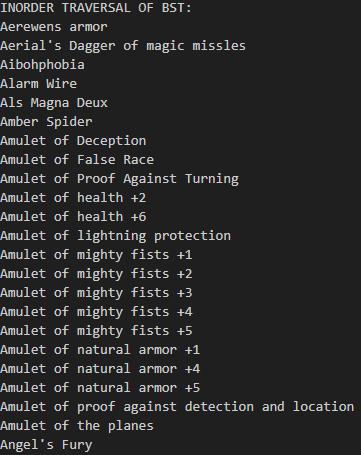
\includegraphics[width=0.45\textwidth]{./imgs/TraversalBST.PNG}}
    \caption{Snippet of BST Insertion Output}
    \label{fig:figure3.9}
\end{figure}

\noindent
It is important to note the time complexity of the traversal. The traversal is $O(n)$, where $n$ represents the number of Nodes in Binary Search Tree. This is because each Node is visited exactly once. In order to print all of the Nodes during the traversal, they have to be visited, meaning the time complexity is $O(n)$. Also, the amount of work done for each Node is constant, meaning that the program just does a print for each Node. This means that the running time is just $O(n)$ when ignoring constant factors.

\subsection{Searching for Items in BST}
\noindent
One of the last functions for the BST class is the search function, which searches for a specific item in the BST. Below is how I implemented this feature.

\begin{figure}[H]
  \centering
  \lstinputlisting[firstline=81, firstnumber=81, lastline=114]{BinarySearchTree/BST.h} 
  \label{fig:figure3.10-part1}
\end{figure}

\begin{figure}[H]
  \centering
  \lstinputlisting[firstline=115, firstnumber=115, lastline=122]{BinarySearchTree/BST.h} 
  \caption{BST Search/Lookup (BST.h)}
  \label{fig:figure3.10-part2}
\end{figure}

\vspace{-1em}
\noindent
This function will return the amount of comparisons it had to do to find the item in the tree (declared on Line 84). The function also has a lot of similarities to the insertion function, like having a curNode which keeps track of the current Node that is being worked on in the loop (Line 85). There is also a string that will keep track of that Node's data (Line 86). The program will traverse the BST until it reaches the correct spot, or until it reaches a NULL Node (the function will try to get the child of a leaf node, but in that case, the item was not found). It checks if the current data is the target item, and if it is, the correct Node has been found and it will break out of the loop (Lines 96-100). If the target item is smaller than the current Node's data in ASCII-terms, it will traverse the current Node's left subtree while printing its path (Lines 102-106). If it is greater than OR EQUAL TO the current Node's data in ASCII-terms, it will traverse the current Node's right subtree while printing its path (Lines 108-112). Like mentioned earlier, if the loop finishs and the current Node is NULL, that means that the item has not been found. In this case, it will print that it wasn't found (Lines 116-119). After this, the function will return with its comparison number (Line 121). In this specific scenario, all items will eventually be found since the "magicitems-find-in-bst.txt" file has items that are definitely in the "magicitems.txt" file. However, even if there were some items that weren't found, the program will still work correctly.

\vspace{0.5em}
\noindent
Below is a snippet of output from this function, displaying the path it took to find the item, including its comparison count (code that printed comparison count at the end of each line is located in main)

\begin{figure}[H] 
    \centering 
    \fbox{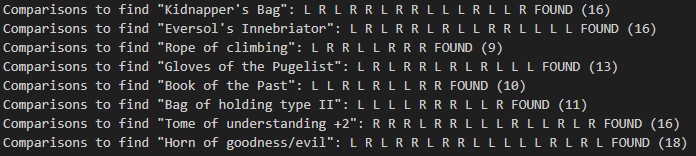
\includegraphics[width=0.97\textwidth]{./imgs/SearchBST.PNG}}
    \caption{Snippet of BST Search Output}
    \label{fig:figure3.11}
\end{figure}

\vspace{2em}
\noindent
It is now time to talk about the time complexity of this BST lookup function. In the absolute worst case scenario, meaning the tree is completely unbalanced, the time complexity could be $O(n)$. This is the case only if the tree resembles a linked list. For example, if there are absolutely no left children and only right children, it would just be a linked list, hence why the lookup time could be $O(n)$. However, it's unlikely this is the case. In cases where the tree is balanced or close to being balanced, the time complexity of BST lookups is $O(\log_2 n)$ or $O(\log n)$ removing constant factors. This is because at each step of the search, around half of the remaining Nodes are eliminated from the possible candidates (it may be approximately half if the tree isn't completely balanced, but if it is perfectly balanced, half of the Nodes would be eliminated each iteration of the loop). This is like a regular binary search, which also has a running time of $O(\log_2 n)$. In both cases, half of the remaining items are removed from the equation entirely, until only one item remains. This is exactly like how a logarithmic function acts, therefore the time complexity for a BST should also be $O(\log_2 n)$.

\subsection{Unload BST}
\noindent
The last functions to explain are the unload functions. Just like the traversal function, there is a public function and private function for the exact same reasons as there was for the other function. To avoid memory leaks, the tree needs to be unloaded once it's done being used. The function call in main is shown below.

\vspace{-1em}
\begin{figure}[H]
  \centering
  \lstinputlisting[firstline=178, firstnumber=178, lastline=179]{main.cpp} 
  \caption{Unload Call (main.cpp)}
  \label{fig:figure3.12}
\end{figure}

\vspace{-0.5em}
\noindent
The public BST class function is named unloadTree, as shown in the function call in main. In the BST class, this function will call the private function named unload. These functions are shown below.

\vspace{-1em}
\begin{figure}[H]
  \centering
  \lstinputlisting[firstline=124, firstnumber=124, lastline=128]{BinarySearchTree/BST.h} 
  \label{fig:figure3.13-part1}
\end{figure}

\vspace{-3em}

\begin{figure}[H]
  \centering
  \lstinputlisting[firstline=131, firstnumber=131, lastline=140]{BinarySearchTree/BST.h} 
  \caption{Unload BST (BST.h)}
  \label{fig:figure3.13-part2}
\end{figure}

\noindent
The private function call in unloadTree shows that the unloading will start by using the root node as its reference (Line 127). The unload function is recursive, unloading all the left subtree and right subtree of each Node before deleting the Node itself (Lines 134-139).

\subsection{Average Comparison Count for BST Lookups}
\noindent
The final thing to talk about is the comparison count for the BST lookups. Even though I've already explained the time complexity of the BST lookup function, it is important to talk about the actual comparison count. The comparison count values can help determine if using a BST is better than just doing a binary search. Below is how I implemented calculating the average comparison count for this program.

\begin{figure}[H]
  \centering
  \lstinputlisting[firstline=174, firstnumber=174, lastline=176]{main.cpp} 
  \caption{Average Comparison Count Calculation (main.cpp)}
  \label{fig:figure3.14}
\end{figure}

\noindent
Before the program reaches the code above, the avg variable will be the sum of all comparisons. To find the average, it needs to be divided by the amount of items that were searched (Line 175). The itemCount integer was also incremented each iteration of file reading to get the amount of items there were in the "magicitems-find-in-bst.txt" file. This calculated average is then printed with a precision of 2 decimal points using the fixed and setprecision manipulators, as explained in the previous assignment (Line 176). 

\vspace{1em}
\noindent
Because I am reading from a set file every time this program is run, the average comparison count will never changed. In this case, it will always be 11.95. Looking at the previous assignment, I would get average comparison counts of binary search around 8-10. Binary Search Tree lookups seem to be worse probably because the tree isn't perfectly balanced. The tree must be slightly off balanced, meaning some lookups will take longer than it could've possibly taken in regular binary search, thus increasing the overall average.

\section{Conclusion}
\setcounter{figure}{0}

\begin{figure}[H] 
    \centering 
    \fbox{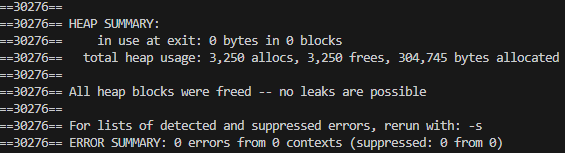
\includegraphics[width=0.98\textwidth]{./imgs/ValgrindOutput.PNG}}
    \caption{Valgrind Output (running command "valgrind ./main")}
    \label{fig:figure4.1}
\end{figure}

\noindent
Wow, this was a wild ride for me. I would like to apologize for this document being nearly 40 pages long, but there was a lot of material to explain. Of course, like last assignment, this assignment was a great learning experience for me, but I think it was an even greater experience than before. I spent most of the time working with the undirected graph implementations. I would work on the linked objects implementation and then not like what I was doing, so I would redo it and then find other optimizations I could've done. It was just a never-ending cycle of redoing my code, and it was messy at times (just look at my commit history). However, I got through it at the end. I used Valgrind a lot again to see if the unloading functions were working properly, and as shown in Figure 4.1, they are since there are no memory leaks.

\vspace{1em}
\noindent
Before going into this assignment, I didn't think I would be writing 20 pages on undirected graphs, but even though it was kind of torturous, I learned a lot doing it. As I was writing this document, I found slight optimizations in my code and I would go back and change some lines. I hope you learned some things too! 

\end{document}
